
\documentclass[a4paper,11pt]{article}
\usepackage[a4paper, margin=8em]{geometry}

% usa i pacchetti per la scrittura in italiano
\usepackage[french,italian]{babel}
\usepackage[T1]{fontenc}
\usepackage[utf8]{inputenc}
\frenchspacing 

% usa i pacchetti per la formattazione matematica
\usepackage{amsmath, amssymb, amsthm, amsfonts}

% usa altri pacchetti
\usepackage{gensymb}
\usepackage{hyperref}
\usepackage{standalone}

% imposta il titolo
\title{Appunti Calcolo Numerico}
\author{Luca Seggiani}
\date{2025}

% disegni
\usepackage{pgfplots}
\pgfplotsset{width=10cm,compat=1.9}

% imposta lo stile
% usa helvetica
\usepackage[scaled]{helvet}
% usa palatino
\usepackage{palatino}
% usa un font monospazio guardabile
\usepackage{lmodern}

% tikz in sans
\tikzset{every picture/.style={/utils/exec={\sffamily}}}

\renewcommand{\rmdefault}{ppl}
\renewcommand{\sfdefault}{phv}
\renewcommand{\ttdefault}{lmtt}

% circuiti
\usepackage{circuitikz}
\usetikzlibrary{babel}

% disponi il titolo
\makeatletter
\renewcommand{\maketitle} {
	\begin{center} 
		\begin{minipage}[t]{.8\textwidth}
			\textsf{\huge\bfseries \@title} 
		\end{minipage}%
		\begin{minipage}[t]{.2\textwidth}
			\raggedleft \vspace{-1.65em}
			\textsf{\small \@author} \vfill
			\textsf{\small \@date}
		\end{minipage}
		\par
	\end{center}

	\thispagestyle{empty}
	\pagestyle{fancy}
}
\makeatother

% disponi teoremi
\usepackage{tcolorbox}
\newtcolorbox[auto counter, number within=section]{theorem}[2][]{%
	colback=blue!10, 
	colframe=blue!40!black, 
	sharp corners=northwest,
	fonttitle=\sffamily\bfseries, 
	title=Teorema~\thetcbcounter: #2, 
	#1
}

% disponi definizioni
\newtcolorbox[auto counter, number within=section]{definition}[2][]{%
	colback=red!10,
	colframe=red!40!black,
	sharp corners=northwest,
	fonttitle=\sffamily\bfseries,
	title=Definizione~\thetcbcounter: #2,
	#1
}

% disponi problemi
\newtcolorbox[auto counter, number within=section]{problem}[2][]{%
	colback=green!10,
	colframe=green!40!black,
	sharp corners=northwest,
	fonttitle=\sffamily\bfseries,
	title=Problema~\thetcbcounter: #2,
	#1
}

% disponi codice
\usepackage{listings}
\usepackage[table]{xcolor}

\definecolor{codegreen}{rgb}{0,0.6,0}
\definecolor{codegray}{rgb}{0.5,0.5,0.5}
\definecolor{codepurple}{rgb}{0.58,0,0.82}
\definecolor{backcolour}{rgb}{0.95,0.95,0.92}

\lstdefinestyle{codestyle}{
		backgroundcolor=\color{black!5}, 
		commentstyle=\color{codegreen},
		keywordstyle=\bfseries\color{magenta},
		numberstyle=\sffamily\tiny\color{black!60},
		stringstyle=\color{green!50!black},
		basicstyle=\ttfamily\footnotesize,
		breakatwhitespace=false,         
		breaklines=true,                 
		captionpos=b,                    
		keepspaces=true,                 
		numbers=left,                    
		numbersep=5pt,                  
		showspaces=false,                
		showstringspaces=false,
		showtabs=false,                  
		tabsize=2
}

\lstdefinestyle{shellstyle}{
		backgroundcolor=\color{black!5}, 
		basicstyle=\ttfamily\footnotesize\color{black}, 
		commentstyle=\color{black}, 
		keywordstyle=\color{black},
		numberstyle=\color{black!5},
		stringstyle=\color{black}, 
		showspaces=false,
		showstringspaces=false, 
		showtabs=false, 
		tabsize=2, 
		numbers=none, 
		breaklines=true
}

\lstdefinelanguage{javascript}{
	keywords={typeof, new, true, false, catch, function, return, null, catch, switch, var, if, in, while, do, else, case, break},
	keywordstyle=\color{blue}\bfseries,
	ndkeywords={class, export, boolean, throw, implements, import, this},
	ndkeywordstyle=\color{darkgray}\bfseries,
	identifierstyle=\color{black},
	sensitive=false,
	comment=[l]{//},
	morecomment=[s]{/*}{*/},
	commentstyle=\color{purple}\ttfamily,
	stringstyle=\color{red}\ttfamily,
	morestring=[b]',
	morestring=[b]"
}

% disponi sezioni
\usepackage{titlesec}

\titleformat{\section}
	{\sffamily\Large\bfseries} 
	{\thesection}{1em}{} 
\titleformat{\subsection}
	{\sffamily\large\bfseries}   
	{\thesubsection}{1em}{} 
\titleformat{\subsubsection}
	{\sffamily\normalsize\bfseries} 
	{\thesubsubsection}{1em}{}

% disponi alberi
\usepackage{forest}

\forestset{
	rectstyle/.style={
		for tree={rectangle,draw,font=\large\sffamily}
	},
	roundstyle/.style={
		for tree={circle,draw,font=\large}
	}
}

% disponi algoritmi
\usepackage{algorithm}
\usepackage{algorithmic}
\makeatletter
\renewcommand{\ALG@name}{Algoritmo}
\makeatother

% disponi numeri di pagina
\usepackage{fancyhdr}
\fancyhf{} 
\fancyfoot[L]{\sffamily{\thepage}}

\makeatletter
\fancyhead[L]{\raisebox{1ex}[0pt][0pt]{\sffamily{\@title \ \@date}}} 
\fancyhead[R]{\raisebox{1ex}[0pt][0pt]{\sffamily{\@author}}}
\makeatother

\begin{document}

% sezione (data)
\section{Lezione del 14-04-25}

% stili pagina
\thispagestyle{empty}
\pagestyle{fancy}

% testo
Abbiamo finora presupposto di avere una serie di punti $(x_j, y_j)$, con $j = 0, ..., k$, tratti da una funzione $f : [a, b] \rightarrow \mathbb{R}$, cioè definita su un certo intervallo $[a, b]$, con $x_j \in [a, b]$ e $y_j = f(x_j) \in \mathbb{R}$.
Da questi punti volevamo ricavare un polinomio $p(x)$ di grado al più $k$ tale che questo interpolasse i punti, cioè verificasse:
$$
p(x_j) = y_j
$$

Da questa configurazione avevamo visto più metodi per il calcolo effettivo di $p(x)$, e avevamo ipotizzato che il modo migliore per aumentarne l'accuratezza, cioè ridurre il massimo della funzione:
$$
r(x) = f(x) - p(x), \quad x \in [a, b]
$$
fosse aumentare $k$.

Questo però aveva diversi aspetti negativi:
\begin{itemize}
	\item Avere $k$ maggiore significa aumentare i punti campionati, cosa che potrebbe non essere sempre fattibile;
	\item Non è detto che $k$ maggiore aumenti l'accuratezza: avevamo visto infatti il \textit{fenomeno di Runge} agli estremi, per cui il limiter dell'errore all'aumentare di $k$ non era zero, cioè:
		$$
		\lim_{k \rightarrow +\infty} |r(x)| \neq 0
		$$
		Avevamo visto un modo per migliorare questa situazione, che era usare nodi non equispaziati ma equispaziati su una circonferenza e proiettati sull'asse reale: questi erano i \textit{nodi di Chebyshev}. 
\end{itemize}

Abbiamo in generale, però, che aumentare il grado $k$ non è la situazione ottimale, e si preferirebbe continuare con funzioni polonomiali di grado basso.
Introduciamo per questo esatto motivo l'\textbf{interpolazione polinomiale a tratti}.

\subsection{Interpolazione polinomiale a tratti}
Decidiamo quindi di spezzare il dominio $[a, b]$ in sottointervalli di tipo $[x_{i - 1}, x_i]$ e di usare in ogni sottointervallo polinomi di grado basso.
In ogni sottointervalloconsideriamo quindi polinomi $p_i(x)$ di grado al più $s < k$ tali che $p_i(x)$ interpola $f$ in $x_{i - 1}$ e $x_i$, cioè:
$$
p_i(x) : [x_{i - 1}, x_i] \rightarrow \mathbb{R}, \quad p_i(x_{i - 1}) = y_{i - 1}, \quad p_i(x_i) = y_i
$$

\newpage

Vediamo quindi alcuni casi particolari di questo tipo di interpolazione al variare di $s$, presa la tabella di punti: 
\begin{table}[h!]
	\center 
	\begin{tabular} { c | c c }
		& $\mathbf{x_j}$ & $\mathbf{y_j}$ \\
		\hline
		$P_0$ & $-13$ & $5$ \\ 
		$P_1$ & $-4$ & $-3$ \\ 
		$P_2$ & $1$ & $2$ \\ 
		$P_3$ & $13$ & $-1$
	\end{tabular}
\end{table}

\subsubsection{$\mathbf{s = 1}$: interpolazione lineare a tratti}
Nel caso più semplice l'interpolazione lineare a tratti si riduce al definire una serie di rette che collegano ogni coppia di punti $x_{i - 1}$, $x_{i}$, in forma:
$$
l_i(x) = m_i(x)+ q_I, \quad i = 1, ..., k 
$$
In particolare, per i 4 punti che abbiamo preso vorremo definire:
\[
	l(x) = 
	\begin{cases}
		l_{1}\left(x\right)=\frac{y_{1}-y_{0}}{x_{1}-x_{0}}\left(x-x_{0}\right)+y_{0}\ , \quad x_{0}\le x < x_{1} \\
		l_{2}\left(x\right)=\frac{y_{2}-y_{1}}{x_{2}-x_{1}}\left(x-x_{1}\right)+y_{1}\ , \quad x_{1}\le x < x_{2} \\
		l_{3}\left(x\right)=\frac{y_{3}-y_{2}}{x_{3}-x_{2}}\left(x-x_{2}\right)+y_{2}\ , \quad x_{2}\le x\le x_{3}
	\end{cases}
\]
direttamente prendendo i fasci di rette in ogni punto $x_0$, $x_1$, $x_2$ (tutti tranne l'ultimo) e imponendo i coefficienti angolari.

Sul grafico, questo tipo di interpolazione (assieme alla derivata prima) avrà l'aspetto:
\begin{center}
	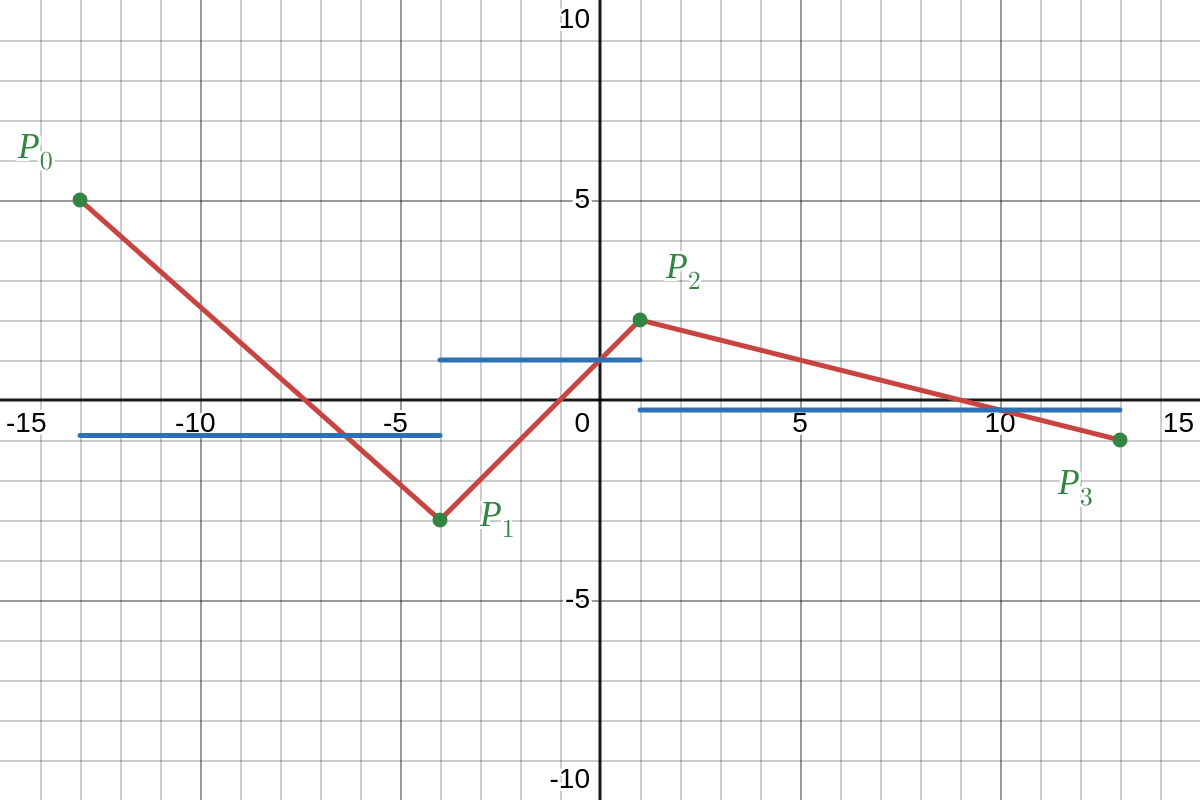
\includegraphics[scale=0.3]{../figures/multipoly_1.png}
\end{center}
da dove si nota chiaramente che con questo approccio la continuità non è assicurata nemmeno al primo grado.

\subsubsection{$\mathbf{s = 2}$: spline quadratiche}
Una soluzione più "liscia" si può avere sfruttando le cosiddette \textbf{spline quadratiche}:
\begin{definition}{Spline quadratica}
	Dati $k + 1$ punti $(x_j, y_j)$ in un intervallo $[a, b]$ con $j = 0, ..., k$ si definisce spline quadratica ($s = 2$) relativa ai $k + 1$ punti la funzione definita a tratti $S_2(x)$ che rispetta le condizioni:
	\begin{enumerate}
		\item $S_2(x)$ è un polinomio di grado 2 se ristretto ad un intervallo $[x_{i - 1}, x_i]$;
		\item $S_2(x_i) = y_i$ per ogni punto $i = 0, ..., k$;
		\item $S_2(x) \in C^1([a, b])$.
	\end{enumerate}
\end{definition}
In questi termini, l'interpolazione lineare a tratti vista finora rappresenta una sorta di interpolazione per \textit{"spline lineari"}, mentre nella prossima sezione vedremo le \textit{spline cubiche}.
Vediamo quindi che le condizioni imposte equivalgono a dire:
\[
	\begin{cases}
		p_i(x_i) = y_i, \quad i = 1, ..., k \\ 
		p_i(x_{i - 1}) = y_{i - 1}, \quad i = 1, ..., k \\ 
		p_i'(x_i) + p_{i + 1}'(x_i), \quad i = 1, ..., k - 1 \\ 
	\end{cases}
\]
cioè abbiamo complessivamente $3k - 1$ condizioni.
Di contro, guardando alla prima condizione si ha che ogni tratto dell'interpolazione avrà forma:
$$
q_i(x) = a_i x^2 + b_i x + c_i, \quad i = 1, ..., k
$$
cioè $3k$ parametri complessivi.

Visto che $3k$ parametri per $3k - 1$ condizioni sono troppi, dobbiamo introdurre un'altra condizione: diciamo che la derivata in $x_0$ deve essere uguale ad un valore fisso $d_0$.

A questo punto basterà trovare $a_i$, $b_i$ e $c_i$ in funzione di $x_{i - 1}$, $x_i$ e la derivata in $x_{i - 1}$ (che chiamiamo $d_{i-1}$), che saranno:
\[
	\begin{cases}
		a_i  =\frac{y_{i}-y_{i-1}}{\left(x_{i-1}-x_{i}\right)^{2}}+\frac{d_{i-1}}{x_{i-1}-x_{i}} \\ 
		b_i = d_{i - 1} -2a_ix_{i-1} \\
		c_i = y_{i}-a_ix_{i}^{2}-b_ix_{i}
	\end{cases}
\]

Calcolando tali valori per ognuno dei $k$ tratti dell'interpolazione si trovano i parametri di ogni quadratica interpolante.

\newpage

Facendo ciò sull'esempio di prima e tracciando il grafico, si ha (assieme alla derivata prima e seconda):
\begin{center}
	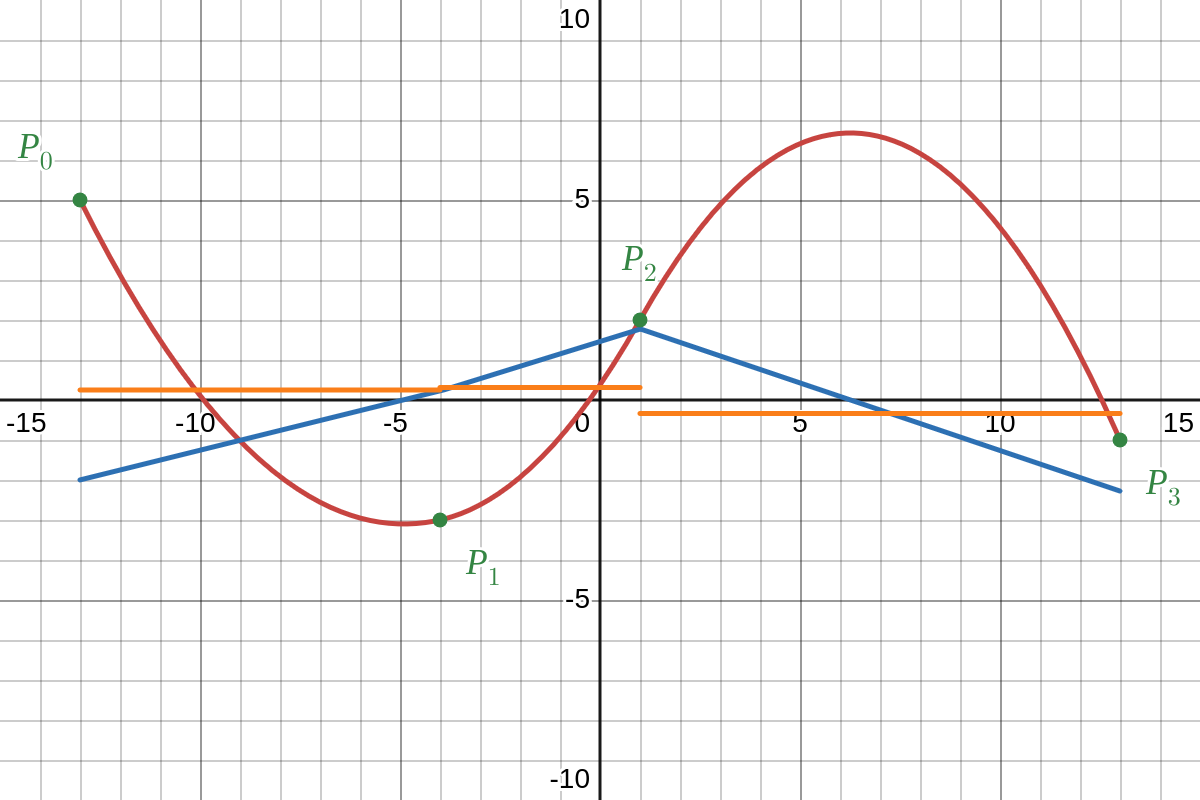
\includegraphics[scale=0.3]{../figures/multipoly_2.png}
\end{center}
da dove notiamo quindi di aver guadagnato la continuità al primo grado, ma ancora non al secondo.
In verità le spline quadratiche non sono molto utili per via delle limitazioni che ci impongono, e vengono usate di rado in contesti reali.
Passiamo quindi a polinomi di grado più alto, molto più di largo uso, cioè $s = 3$.

\subsubsection{$\mathbf{s = 3}$: spline cubica}
Una soluzione ancora più "liscia" si può quindi avere sfruttando le cosiddette \textbf{spline cubiche}.
Queste sono il tipo più comune di spline, e vengono usate in svariati contesti, fra cui ad esempio per tracciare linee "smussate" in computer grafica.

Definiamo quindi:
\begin{definition}{Spline cubica}
	Dati $k + 1$ punti $(x_j, y_j)$ in un intervallo $[a, b]$ con $j = 0, ..., k$ si definisce spline cubica ($s = 3$) relativa ai $k + 1$ punti la funzione definita a tratti $S_3(x)$ che rispetta le condizioni:
	\begin{enumerate}
		\item $S_3(x)$ è un polinomio di grado 3 se ristretto ad un intervallo $[x_{i - 1}, x_i]$;
		\item $S_3(x_i) = y_i$ per ogni punto $i = 0, ..., k$;
		\item $S_3(x) \in C^2([a, b])$.
	\end{enumerate}
\end{definition}
Vediamo quindi che le condizioni imposte equivalgono a dire:
\[
	\begin{cases}
		p_i(x_i) = y_i, \quad i = 1, ..., k \\ 
		p_i(x_{i - 1}) = y_{i - 1}, \quad i = 1, ..., k \\ 
		p_i'(x_i) + p_{i + 1}'(x_i), \quad i = 1, ..., k - 1 \\ 
		p_i''(x_i) + p_{i + 1}''(x_i), \quad i = 1, ..., k - 1 \\ 
	\end{cases}
\]
con una riga in più di condizioni rispetto al caso quadratico dato dal salto da continuità $C^1$ a $C^2$, cioè abbiamo complessivamente $4k - 2$ condizioni.
Di contro, guardando alla prima condizione si ha che ogni tratto dell'interpolazione avrà forma:
$$
c_i(x) = a_i x^3 + b_i x^2 + c_i x + d_i, \quad i = 1, ..., k
$$
cioè $4k$ parametri complessivi.

Come nel caso quadratico, visto che $4k$ parametri per $4k - 2$ condizioni sono troppi, dovremo introdurre 2 nuove condizioni, che modificheranno il tipo di problema che andremo a risolvere:
\begin{itemize}
	\item \textbf{Spline naturale:} si considera questo tipo di spline quando non si ha alcun tipo di informazione oltre i punti da interpolare. In questo caso si assume quindi:
		$$
		p_1''(x_0) = p_k''(x_k) = 0
		$$
		cioè derivata seconda nulla agli estremi di interpolazione $x_0 = a$ e $x_k = b$ di $[a, b]$;
	\item \textbf{Spline periodica:} quando si ritiene che la funzione da approssimare sia periodica, si possono adottare le condizioni:
		$$
		p_1''(x_0) = p_k''(x_k), \quad p_1'(x_0) = p_k'(x_k)
		$$
	\item \textbf{Spline vincolata:} infine, se si conoscono le derivate prime negli estremi di interpolazione $x_0 = a$ e $x_k = b$ si possono imporre le condizioni:
		$$
		p_1'(x_0) = f'(x_0), \quad p_k'(x_k) = f'(x_k)
		$$
		
		Un altro tipo di spline vincolata potrebbe essere quello da usare nel caso in cui si conoscono derivata prima e seconda nel primo estremo di interpolazione $x_0 = a$.
		In questo caso si impongono le condizioni:
		$$
		p_1'(x_0) = f'(x_0) \quad p_1''(x_0) = f''(x_0)
		$$
		Questo equivale al caso che abbiamo considerato per la spline quadratica (chiamando $f'(x_0) = d_0$ e $f''(x_0) = s_0$), salvo aver dovuto introdurre un ulteriore grado di derivazione.
\end{itemize}

In ogni caso, per punti equispaziati i può dimostrare il seguente teorema:
\begin{theorem}{Esistenza di spline cubiche}
	Presi $x_0, ..., x_k$ nodi equispaziati su un intervallo $[a, b]$, cioè:
	$$
	x_i = a + ih, \quad h = \frac{b - a}{k}, \quad i = 0, ..., k
	$$
	e le valutazioni $y_0, ..., y_k$ di una certa funzione $f(x)$ nei nodi $x_i$, esiste unica la spline naturale $S_3(x)$ passante per i punti $(x_i, y_i)$, $i = 0, ..., k$.
\end{theorem}

Vediamo quindi due procedimenti di calcolo per due dei casi appena definiti, cioè il primo (spline naturale )e l'ultimo (spline vincolata in $x_0$).
Le formule per il calcolo degli altri due casi saranno in qualche modo ricavate in modo equivalente a quelle del primo caso.
\begin{itemize}
	\item Un primo approccio può essere quello di risolvere ognuno dei $k$ sottoproblemi di interpolazione fra $x_{i - 1}$ e $x_i$ applicando l'interpolazione di Hermite, e portandosi dietro le derivate prime $m_i$ (che ancora non conosciamo), interpretate come $f'(x_i)$.
		Si determinano quindi gli $m_i$ imponendo le condizioni sulla derivata seconda agli estremi (abbiamo detto la \textit{condizione naturale}).
	
		Presi quindi punti equispaziati come sopra, cioè:
		$$
		x_i = a + ih, \quad h = \frac{b - a}{k}, \quad i = 0, ..., k
		$$
		questo procedimento porta alla formazione di spline del tipo:
		$$
		p_i(x) = \left[ f(x_{i - 1}) + \left( m_{i - 1} + \frac{2 f(x_{i - 1})}{h} \right) (x - x_{i - 1})  \right] \left( \frac{x - x_i}{h} \right)^2
		$$
		$$
		+ \left[ f(x_{i}) + \left( m_{i} - \frac{2 f(x_{i })}{h} \right) (x - x_{i})  \right] \left( \frac{x - x_{i - 1}}{h} \right)^2
		$$
		direttamente dall'interpolazione di Hermite, con gli $m_i$ soluzioni del seguente sistema lineare:
		$$
		\begin{pmatrix}
			2 & 1 & 0 & ... & 0 \\ 
			1 & 4 & 1 & ... & 0 \\
			0 & \ddots & \ddots & \ddots & 0 \\
			0 & ... & 1 & 4 & 1 \\
			0 & ... & 0 & 1 & 2
		\end{pmatrix}
		\begin{pmatrix}
			m_0 \\ m_1 \\ m_2 \\ \vdots \\ m_k
		\end{pmatrix}
		=
		\frac{3}{h}
		\begin{pmatrix}
			f(x_1) - f(x_0) \\
			f(x_2) - f(x_0) \\
			f(x_3) - f(x_1) \\
			\vdots \\
			f(x_{k-1}) - f(x_{k-2}) \\
			f(x_k) - f(x_{k-1})
		\end{pmatrix}
		$$
		da dove si nota la matrice $A$ a \textit{˝striscia"}, data dall'interdipendenza fra i tratti della spline.

	In particolare, procediamo con la dimostrazione.
	Vorremo interpolare ogni tratto $x_{i - 1}$, $x_i$ con un polinomio $p_i(x)$ di terzo grado che rispetti:
	\[
		\begin{cases}
			p_i(x_{i - 1}) = f(x_{i - 1}) \\
			p_i(x_i) = f(x_i) \\
			p_i(x_{i - 1}) = m_{i - 1} \\
			p_i(x_i) = m_1
		\end{cases}
	\]
	dove i $k + 1$ valori $m_0, m_1, ..., m_k$ sono le derivate prime che ancora non conosciamo.
	Avremo quindi da Hermite che vorremmo prendere le basi di Lagrange:
	$$
	e_{i-1}(x) = \frac{x - x_i}{x_{i-1} - x_i}, \quad e_i(x) = \frac{x - x_{i-1}}{x_i - x_{i-1}}
	$$
	e quindi le basi di Hermite:
	\[
		\begin{cases}
			h_{00}\left(x\right) = (1 - 2e_{i - 1}'(x_{i - 1})(x - x_{i-1}))e_{i-1}^2(x) = \left(1+\frac{2}{x_{i}-x_{i-1}}\left(x-x_{i-1}\right)\right)\left(\frac{x-x_{i}}{x_{i}-x_{i-1}}\right)^{2}	\\

			h_{01}\left(x\right) = (1 - 2e_{i}'(x_i)(x - x_i))e_i^2(x) =\left(1-\frac{2}{x_{i}-x_{i-1}}\left(x-x_{i}\right)\right)\left(\frac{x-x_{i-1}}{x_{i}-x_{i-1}}\right)^{2} \\

			h_{10}\left(x\right) = (x - x_{i - 1})e_{i-1}^2(x) = \left(x-x_{i-1}\right)\left(\frac{x-x_{i}}{x_{i}-x_{i-1}}\right)^{2} \\

			h_{11}\left(x\right) = (x - x_{i})e_{i}^2(x) = \left(x-x_{i}\right)\left(\frac{x-x_{i-1}}{x_{i}-x_{i-1}}\right)^{2}
		\end{cases}
	\]
	da cui il polinomio interpolante finale è:
	$$
	p_i\left(x\right)=h_{00}\left(x\right)y_{0}+h_{01}\left(x\right)y_{1}+h_{10}\left(x\right)m_{0}+h_{11}\left(x\right)m_{1}
	$$
	$$
	=\left(y_{0}+\left(m_{0}+\frac{2y_{0}}{x_{i}-x_{i-1}}\right)\left(x-x_{i-1}\right)\right)\left(\frac{x-x_{i}}{x_{i}-x_{i-1}}\right)^{2}
	$$
	$$
	+\left(y_{1}+\left(m_{1}-\frac{2y_{1}}{x_{i}-x_{i-1}}\right)\left(x-x_{i}\right)\right)\left(\frac{x-x_{i-1}}{x_{i}-x_{i-1}}\right)^{2}
	$$
	che posto $x_i - x_{i - 1} = h$, e $y_i = f(x_i)$, è esattamente quanto dato prima.
	
	A questo punto resta da ricavare il sistema lineare.
	Per fare ciò calcoliamo la derivata seconda del polinomio interpolante nei punti $x_{i - 1}$ e $x_i$:
	$$
	p_i''(x_{i - 1}) = \frac{6\left(y_{1}-y_{0}\right)}{\left(x_{i}-x_{i-1}\right)^{2}}-\frac{4m_{0}+2m_{1}}{x_{i}-x_{i-1}}
	$$
	$$
	p_i''(x_i) = \frac{2m_{0}+4m_{1}}{x_{i}-x_{i-1}}-\frac{6\left(y_{1}-y_{0}\right)}{\left(x_{i}-x_{i-1}\right)^{2}}
	$$

	Avremo allora le condizioni della spline cubica naturale, cioè derivata seconda nulla agli estremi:
	\[
		\begin{cases}	
			p_1''(x_0) = 0 \implies 2m_0 + m_1 = \frac{3}{h} \left( f(x_1) - f(x_0) \right) \\
			p_k''(x_k) = 0 \implies 2m_k + m_{k - 1} = \frac{3}{h} \left( f(x_k) - f(x_{k - 1}) \right) \\
		\end{cases}
	\]
	e derivate seconde continue nei punti intermedi:
	$$
		p_i''(x_i) = p_{i+1}''(x_{i}) \implies m_{i - 1} + 4 m_i + m_{i + 1} = \frac{3}{h} f(x_{i + 1}) - f(x_{i - 1})
	$$
	da cui il sistema lineare che corredava la forma del polinomio di Hermite, e quindi la tesi. \qed

	\item Se si vuole imporre il vincolo "a sinistra" della derivata prima e seconda, si può procedere in maniera analoga a quanto fatto nel caso quadratico, cioe prendere i tratti polinomiali:
		$$
		c_i(x) = a_i x^3 + b_i x^2 + c_i x + d_i, \quad i = 1, ..., k
		$$
		e trovare gli $a_i$, $b_i$, $c_i$ e $d_i$ in funzione di $x_{i - 1}$, $x_i$ e le due derivate consecutive in $x_{i - 1}$ (che chiamiamo $d_{i - 1}$ e $s_{i- 1}$, rispettivamente primo e secondo grado).
		
		Visto che trovare direttamente i quattro problemi può essere difficile, decidiamo invece di trovare le 4 basi ortogonali $b_1$, $b_2$, $b_3$ e $b_4$ (di cui le prime 3 equivalenti a quelle di Hermite, e l'ultima corrispondente alla condizione derivata seconda in $x_{i - 1}$), che rispettano quindi le condizioni:
		$$
		b_1 : 
			\begin{cases}
				b_1(x_{i - 1}) = 1 \\
				b_1(x_i) = 0 \\
				b_1'(x_{i - 1}) = 0 \\
				b_1''(x_{i - 1}) = 0 \\
			\end{cases}, \quad
		b_2 : 
			\begin{cases}
				b_2(x_{i - 1}) = 0 \\
				b_2(x_i) = 1 \\
				b_2'(x_{i - 1}) = 0 \\
				b_2''(x_{i - 1}) = 0 \\
			\end{cases}
		$$

		$$
		b_3 : 
			\begin{cases}
				b_3(x_{i - 1}) = 0 \\
				b_3(x_i) = 0 \\
				b_3'(x_{i - 1}) = 1 \\
				b_3''(x_{i - 1}) = 0 \\
			\end{cases}, \quad
		b_4 : 
			\begin{cases}
				b_3(x_{i - 1}) = 0 \\
				b_3(x_i) = 0 \\
				b_3'(x_{i - 1}) = 0 \\
				b_3''(x_{i - 1}) = 1 \\
			\end{cases}
		$$

		Queste si potranno ricavare, direttamente dall'imposizione delle condizioni, come:
		\begin{enumerate}
			\item $b_{1}\left(x,x_{i-1},x_{i}\right)=a_{b1}\left(x_{i-1},x_{i}\right)x^{3}+b_{b1}\left(x_{i-1},x_{i}\right)x^{2}+c_{b1}\left(x_{i-1},x_{i}\right)x+d_{b1}\left(x_{i-1},x_{i}\right)$,
				con:
				\begin{itemize}
					\item $a_{b1}\left(x_{i-1},x_{i}\right)=\frac{1}{\left(x_{i-1}-x_{i}\right)^{3}}$;
					\item $b_{b1}\left(x_{i-1},x_{i}\right)=-3a_{b1}\left(x_{i-1},x_{i}\right)x_{i-1}$;
					\item $c_{b1}\left(x_{i-1},x_{i}\right)=3a_{b1}\left(x_{i-1},x_{i}\right)x_{i-1}^{2}$;
					\item $d_{b1}\left(x_{i-1},x_{i}\right)=1-a_{b1}\left(x_{i-1},x_{i}\right)x_{i-1}^{3}$.
				\end{itemize}
			\item Questa è banalmente $b_{2} \left( x, x_{i-1}, x_{i} \right) = 1 - b_{1}\left(x,x_{i-1},x_{i}\right)$;
			\item $b\left(x,x_{i-1},x_{i}\right)=a_{b3}\left(x_{i-1},x_{i}\right)x^{3}+b_{b3}\left(x_{i-1},x_{i}\right)x^{2}+c_{b3}\left(x_{i-1},x_{i}\right)x+d_{b3}\left(x_{i-1},x_{i}\right)$,
				con:
				\begin{itemize}
					\item $a_{b3}\left(x_{i-1},x_{i}\right)=\frac{x_{i-1}-x_{i}}{\left(x_{i}-x_{i-1}\right)^{3}}$;
					\item $b_{b3}\left(x_{i-1},x_{i}\right)=-3a_{b3}\left(x_{i-1},x_{i}\right)x_{i-1}$;
					\item $c_{b3}\left(x_{i-1},x_{i}\right)=1+3a_{b3}\left(x_{i-1},x_{i}\right)x_{i-1}^{2}$;
					\item $d_{b3}\left(x_{i-1},x_{i}\right)=-a_{b3}\left(x_{i-1},x_{i}\right)x_{i-1}^{3}-x_{i-1}$.
				\end{itemize}
			\item $b\left(x,x_{i-1},x_{i}\right)=a_{b4}\left(x_{i-1},x_{i}\right)x^{3}+b_{b4}\left(x_{i-1},x_{i}\right)x^{2}+c_{b4}\left(x_{i-1},x_{i}\right)x+d_{b4}\left(x_{i-1},x_{i}\right)$,
				con:
				\begin{itemize}
					\item $a_{b4}\left(x_{i-1},x_{i}\right)=\frac{\left(x_{i}-x_{i-1}\right)^{2}}{2\left(x_{i-1}-x_{i}\right)^{3}}$;
					\item $b_{b4}\left(x_{i-1},x_{i}\right)=\frac{1}{2}-3a_{b4}\left(x_{i-1},x_{i}\right)x_{i-1}$;
					\item $c_{b4}\left(x_{i-1},x_{i}\right)=3a_{b4}\left(x_{i-1},x_{i}\right)x_{i-1}^{2}-x_{i-1}$;
					\item $d_{b4}\left(x_{i-1},x_{i}\right)=\frac{1}{2}x_{i-1}^{2}-a_{b4}\left(x_{i-1},x_{i}\right)x_{i-1}^{3}$.
				\end{itemize}
		\end{enumerate}

		A questo punto basterà definire ogni tratto polinomiale $c_i$ come:
$$
c_{i}\left(x\right)=b\left(x,x_{i-1},x_{i}\right)y_{i-1}+b\left(x,x_{i-1},x_{i}\right)y_{i}+b\left(x,x_{i-1},x_{i}\right)d_{i-1}+b\left(x,x_{i-1},x_{i}\right)s_{i-1}\
$$
dove gli $d_{i-1}$ e $s_{i-1}$ sono rispettivamente la derivata prima e seconda in ogni punto, data per il punto $x_0$ e ricavata dal tratto precedente per ogni tratto successivo.

\newpage

Un interpolazione di questo tipo per l'esempio considerato nelle scorse sezioni ha l'aspetto, prese $d_{0} = 1$ e $s_{0} = -1$ e tracciate derivata prima e seconda:
\begin{center}
	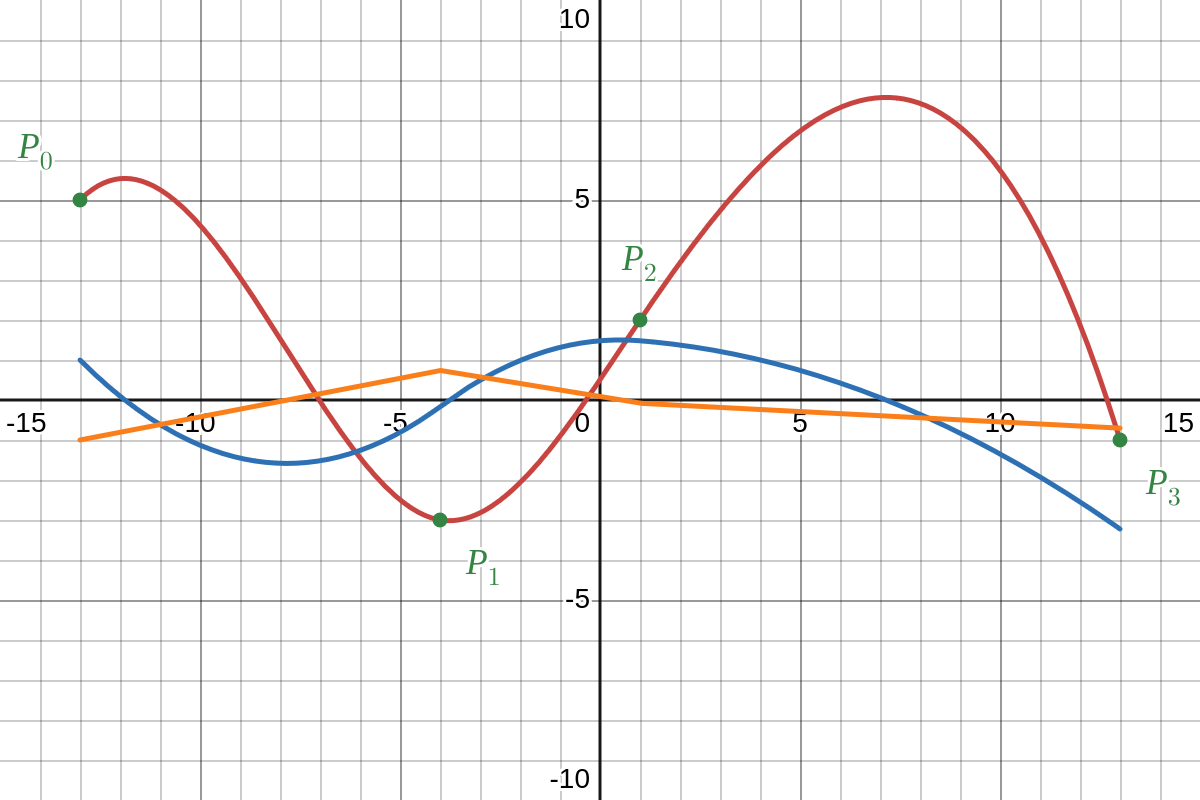
\includegraphics[scale=0.3]{../figures/multipoly_3.png}
\end{center}
da dove notiamo che la derivata fino al secondo grado resta continua, da cui la condizione 3 è rispettata.

Vediamo che in verità si può risolvere in qualche modo anche lo scorso tipo di problema con questo metodo, semplicemente imponendo $s_0 = 0$ e cercando $d_0$ perché risulti $s_k = 0$.
Nell'esempio, questo si ottiene per $d_0 \approx -1.574$, con relativo grafico:
\begin{center}
	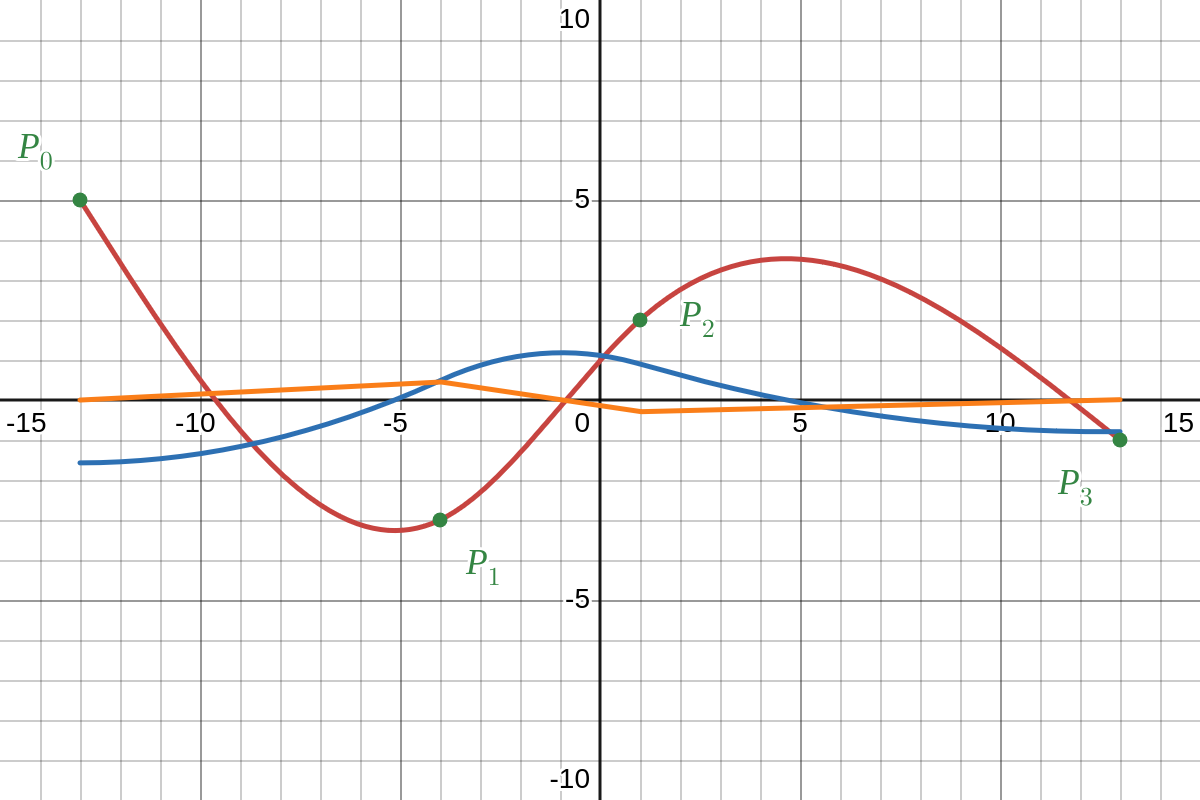
\includegraphics[scale=0.3]{../figures/multipoly_nat.png}
\end{center}
\end{itemize}

Esempi di questi tipi di interpolazione si possono trovare sempre su Desmos, al link \url{https://www.desmos.com/calculator/gm1idqauiy} (da qui sono state generate le figure).

\subsection{Approssimazione ai minimi quadrati}
Un altro approccio per l'approssimazione di insiemi di punti, specialmente nel caso questi siano imponenti in dimensioni, può essere dato dall'\textbf{approssimazione ai minimi quadrati}.

Un caso banale di questo tipo di approssimazione può essere quello della \textit{regressione lineare}: dato un insieme di $k + 1$ punti $(x_j, y_j)$, si cerca la retta che minimizza la distanza quadratica da ogni punto.
In qusto caso la retta prende il nome di \textbf{funzione modello}.

Generalizziamo quindi questo approssimazione in 2 direzioni:
\begin{itemize}
	\item Ammettiamo che si abbiano più punti che funzioni modello (che possiamo intendere come le basi polinomiali usate finora);
	\item Amettiamo l'utilizzo di funzioni modello non polinomiali.
\end{itemize}

Formalmente, quindi, dati $k + 1$ punti $(x_0, y_0), ..., (x_k, y_k)$ punti con $y_j = f(x_j)$ e $m + 1$ funzioni modello $G_0(x), ..., G_m(x)$ con $m \leq x$ cercheremo l'approssimante $\Phi(x) \approx f(x)$ della forma:
$$
\Phi(x) = \sum_{i = 0}^m G_i(x) \cdot c_i, \quad c_i \in \mathbb{R}
$$
con $c_i$ da trovare, cioè la combinazione lineare ottima (definiremo cosa significa ottima fra poco) delle funzioni modello.

\begin{itemize}
	\item 
Ad esempio, la regressione lineare quella data dalle funzioni modello:
$$
G_0(x) = 1, \quad G_1(x) = x
$$
approssimante $k + 1 = \#$ punti nel grafico;
\item Potremmo avere altri tipi di funzioni modello.
Ad esempio potremmo avere:
	$$
G_0(x) = e^{2x}, \quad G_1(x) = \sin\left( \frac{x}{2} \right), \quad G_2(x) = \frac{1}{3x^2 + 4}
$$
In questo caso l'approssimante avrebbe una forma del tipo:
$$
\Phi(x) = c_0 e^{2x} + c_1 \sin \left( \frac{x}{2} \right) + \frac{c_2}{3x^2 + 4}
$$
\end{itemize}

\par\smallskip

A questo punto il problema è capire cosa significa dire che $\Phi(x)$ passa \textit{"vicino"} ai punti $(x_j, y_j)$, cioè qual'è la funzione da ottimizzare per trovare i $c_i$ ottimi in modo che risulti $\Phi(x) \approx f(x)$.
Dobbiamo quindi definire una qualche funzione di errore $\psi(c_0, ..., c_m) : \mathbb{R}^{m + 1} \rightarrow \mathbb{R}^+$.

Vediamo come definire tale funzione.
\begin{itemize}
	\item Un primo approccio potrebbe essere il semplice \textit{scarto}:
		$$
		\psi(c_0, ..., c_m) = \sum_{i = 0}^k \left( \Phi(x_i) - y_i \right)
		$$
		Questa ha il problema di poter dare cancellazione, cioè errori di punti diversi potrebbero annullarsi, per dare valori di $\psi$ bassi quando in realtà la funzione è molto lontana da $f(x)$;
	\item Un approccio migliore è quindi quello di prendere lo \textit{scarto assoluto}:
		$$
		\psi(c_0, ..., c_m) = \sum_{i = 0}^k \Big| \Phi(x_i) - y_i \Big|
		$$
		In questo caso non soffriremo di cancellazione, ma avremo il problema che $\psi$ non è differenziabile (si avranno punti angolosi dati dal valore assoluto);
	\item L'approccio migliore risulta quindi:
		$$
		\psi(c_0, ..., c_m) = \sum_{i = 0}^k \left( \Phi(x_i) - y_i \right)^2
		$$
		cioè lo \textit{scarto quadratico}, che risolve sia i problemi della cancellazione che della continuità $C^1$.
\end{itemize}

Il metodo dei minimi quadrati consisterà quindi nello scegliere:
$$
c = 
\begin{pmatrix}
	c_0 \\ c_1 \\ \vdots \\ c_m
\end{pmatrix}
\in \mathbb{R}^{m + 1}
$$
tale che:
$$
c = \min_{c \in \mathbb{R}^{m + 1}} \psi(c)
$$
cioè $c$ è punto di minimo di $\psi(c)$.

Dovremo qunidi minimizzare:
$$
\psi(c) = \sum_{i = 0}^k \left( \Phi(x_i) - y_i \right)^2 = \sum_{i = 0}^k \left( \sum_{j = 0}^m c_j \cdot G_j(x_i) - y_i \right)^2
$$
cioè in forma matriciale, posti:
$$
A =
\begin{pmatrix}
	G_0(x_0) & G_1(x_0) & ... & G_m(x_0) \\
	\vdots & & & \vdots \\
	G_0(x_0) & G_1(x_1) & ... & G_m(x_k)
\end{pmatrix}, \quad
c =
\begin{pmatrix}
	c_0 \\ \vdots \\ c_m
\end{pmatrix}, \quad
b = 
\begin{pmatrix}
	y_0 \\ \vdots \\ y_k
\end{pmatrix}
$$
con $A \in \mathbb{R}^{ (k + 1) \times (m + 1) }$, $c \in \mathbb{R}^{m + 1}$, $b \in \mathbb{R}^{k + 1}$, equivale a:
$$
\psi(c) = \sum_{i = 0}^k \left( (Ac)_i - b_i \right)^2 = \Big| Ac - b \Big|_2^2
$$

Stiamo quindi minimizzando la norma quadratica del residuo di $Ac = b$, che dalle dimensioni della matrice $A$ e i vettori $c$ e $b$ è un sistema sovradeterminato (più equazioni che incognite):
$$
c^* = \min_{c \in \mathbb{R}^{m + 1}} |Ac - b|_2
$$
Possiamo quindi risolvere interpretando il sistema come uno di quelli visti in 11.1, quindi sfruttando le \textbf{equazioni normali} o la \textbf{decomposizione QR}.

\end{document}
